\section{Appendix}

	\begin{frame}[label={frame:appendix:ore}]

		\frametitle{OPE / ORE schemes}

		\begin{table}
			\begin{adjustbox}{width=\linewidth}
				\begin{tabular}{ l c c c c c }

					\toprule

					\multirow{2}{*}{Scheme}						& \multicolumn{2}{c}{ Primitive usage}																	& Ciphertext size,																	& Leakage																\\ \cline{2-3}
					\rule{0pt}{10pt}							& Encryption												& Comparison								& or state size																	& (in addition to inherent total order)										\\

					\toprule

					BCLO \cite{crypt-db-ope}					& $\bm{n}$ \textbf{HG}										& none										& $2n$																				& \textbf{$\approx$ Top half of the bits}								\\

					\midrule

					CLWW \cite{practical-ore}					& $n$ PRF 													& none										& $2n$																				& \textbf{Most-significant differing bit}								\\

					\midrule

					\multirow{3}{*}{Lewi-Wu \cite{lewi-ore}}	& \boldmath{} $\nicefrac{2n}{d}$ \unboldmath{} \textbf{PRP}	& \multirow{3}{*}{$\frac{n}{2d}$ Hash}		& \multirow{3}{*}{$\frac{n}{d} \left(\lambda + n + 2^{d + 1} \right) + \lambda$}	& \multirow{3}{*}{Most-significant differing block}						\\
																& $2 \frac{n}{d} \left( 2^d + 1 \right)$ PRF				&											&																					&																		\\
																& $\frac{n}{d} 2^d$ Hash									&											&																					&																		\\

					\midrule

					\multirow{3}{*}{CLOZ \cite{adam-ore-v2}}	& $n$ PRF													& \multirow{3}{*}{$\bm{n^2}$ \textbf{PPH}}	& \multirow{3}{*}{$n \cdot h$}														& \multirow{3}{*}{Equality pattern of most-significant differing bit}	\\
																& $n$ PPH													&											&																					&																		\\
																& 1 PRP														&											&																					&																		\\

					\midrule

					FH-OPE \cite{fh-ope}						& 1 Traversal												& 3 Traversals									& $\bm{3 \cdot n \cdot N}$															& Insertion order													\\

					\bottomrule

				\end{tabular}
			\end{adjustbox}
			\captionsetup{justification=justified}
			\caption{
				\cite[Table 1]{ore-benchmark-17}.
				Primitive usage by OPE / ORE schemes.
				Ordered by security rank --- most secure below.
				$n$ is the input length in bits, $d$ is a block size for Lewi-Wu \cite{lewi-ore} scheme, $\lambda$ is a PRF output size, $N$ is a total data size, \textbf{HG} is a hyper-geometric distribution sampler, \textbf{PPH} is a property-preserving hash with $h$-bit outputs built with bilinear maps and \textbf{bolded} are weak points of the schemes.
			}
		\end{table}

		\begin{flushright}
			\hyperlink{frame:ore}{\beamerreturnbutton{Back to ORE}}
		\end{flushright}

	\end{frame}

	\begin{frame}[label={frame:appendix:protocols}]

		\frametitle{Range query protocols}

		\begin{table}
			\begin{adjustbox}{width=\linewidth}
				\begin{tabular}{ l c c c c c }

					\toprule

					\multirow{2}{*}{Protocol}						& \multicolumn{2}{c}{ {\IO} requests}																													& \multirow{2}{*}{ Leakage}	& \multicolumn{2}{c}{ Communication (result excluded)}													\\ \cline{2-3} \cline{5-6}
					\rule{0pt}{10pt}								& Construction										& Query																								&							& Construction										& Query 											\\

					\toprule

					{\BPlus} tree with ORE							& $\log_B \frac{N}{B}$								& $\log_B \frac{N}{B} + \frac{r}{B}$																& \textbf{Same as ORE}		& $1$												& $1$												\\
					\midrule

					Kerschbaum \cite{florian-protocol}				& $\bm{\frac{N}{B}}$								& $\log_2 \frac{N}{B} + \frac{r}{B}$																& \textbf{Total order}		& $\log_2 N$										& $\log_2 N$										\\

					\midrule

					POPE \cite{pope} warm							& \multirow{2}{*}{ $1$}								& $\log_L \frac{N}{B} + \frac{r}{B}$																& \textbf{Partial order}	& \multirow{2}{*}{ $1$}								& $\log_L N$										\\

					POPE \cite{pope} cold							& 													& $\bm{{\nicefrac{N}{B}}}$																			& Fully hiding				& 													& $\bm{N}$											\\

					\midrule

					Logarithmic-BRC \cite{practical-range-search}	& \textbf{---}										& $\bm{r}$																							& Same as SSE				& \textbf{---}										& $\log_2 N$										\\

					\midrule

					\multirow{2}{*}{ORAM}							& \multirow{2}{*}{ $\bm{{ \log^2 \frac{N}{B} }}$}	& \multirow{2}{*}{ $\bm{{ \log_2 \frac{N}{B} \left( \log_B \frac{N}{B} + \frac{r}{B} \right) }}$}	& Fully hiding				& \multirow{2}{*}{ $\bm{{ \log^2 \frac{N}{B} }}$}	& \multirow{2}{*}{ $\bm{{ \log^2 \frac{N}{B} }}$}	\\
																	&													&																									& (access pattern)			&													&													\\

					\bottomrule

				\end{tabular}
			\end{adjustbox}
			\captionsetup{justification=justified}
			\caption{
				\cite[Tables 2]{ore-benchmark-17}.
				Performance of the range query protocols.
				Ordered by security rank --- most secure below.
				$N$ is a total data size, $B$ is an I/O page size, $L$ is a POPE tree branching factor, $r$ is the result size in records and \textbf{bolded} are weak points of the protocols.
			}
		\end{table}

	\begin{flushright}
		\hyperlink{frame:ore}{\beamerreturnbutton{Back to ORE}}
	\end{flushright}

	\end{frame}

	\begin{frame}[label={frame:appendix:plot}]

		\frametitle{One of the experimental results}

		\begin{figure}[h]
			\centering
			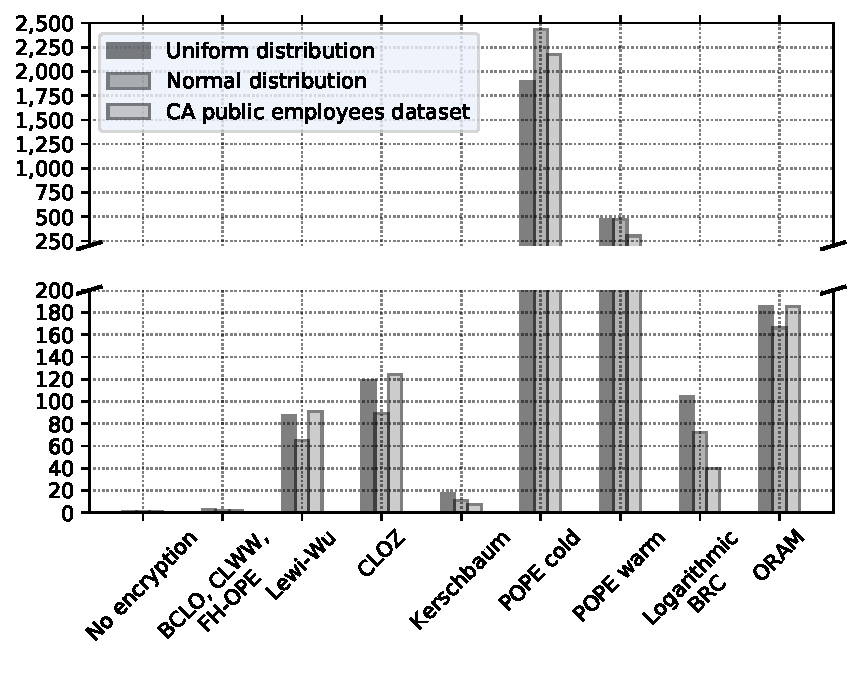
\includegraphics[width=0.6\textwidth]{protocol-charts-qios}
			\caption{
				Query stage number of I/O requests \\
				\hyperlink{frame:ore}{\beamerreturnbutton{Back to ORE}}
			}
		\end{figure}

	\end{frame}

	\begin{frame}[label={frame:appendix:oram}]

		\frametitle{Access pattern and ORAM}

		\justifying%

		\textbf{Access pattern} is a sequence of memory accesses \oramProgram{}, where each access consists of the memory \emph{location} $o$, read \oramRead{} or write \oramWrite{} \emph{operation} and the \emph{data} $d$ to be written.

		Oblivious RAM (ORAM) is a mechanism that hides the accesses pattern.
		More formally, \oram{} is a protocol between the client \client{} (who accesses) and the server \server{} (who stores), with a guarantee that the view of the server is indistinguishable for any two sequences of the same lengths.

		\begin{columns}[T]
			\column{0.475\textwidth}

				\[
					\begin{split}
						\abs{\oramProgram_1}					& = \abs{\oramProgram_2}							\\
						\textsc{View}_\server (\oramProgram_1)	& \cindist \textsc{View}_\server (\oramProgram_2)
					\end{split}
				\]

			\column{0.475\textwidth}

				\procedure[linenumbering]{\oram{} protocol}{
					\textbf{Client \client}											\>														\> \textbf{Server \server}	\\
					%
					\oramProgram{} = \left. (\oramRead, i, \bot) \right|_{i = 1}^5	\> 														\>							\\
					%
					\text{(client state)}											\> \sendmessageboth*[6em]{\algo{ORAM}{\oramProgram}}	\> \text{(server state)}	\\
					%
					\{ d_1, d_2, d_3, d_4, d_5 \}									\>														\>
				}

		\end{columns}

		\vspace*{1ex}

		Square Root ORAM \cite{oram-theory}, Hierarchical ORAM \cite{oram-original}, Binary-Tree ORAM \cite{binary-tree-oram}, Interleave Buffer Shuffle Square Root ORAM \cite{shortest-path-oram}, TP-ORAM \cite{tp-oram}, \textbf{PathORAM} \cite{path-oram} and TaORAM \cite{taostore}.
		\alert{ORAM incurs at least logarithmic overhead in the number of stored records. \cite{oram-original}}

		\begin{flushright}
			\hyperlink{frame:epsolute-motivation}{\beamerreturnbutton{Back to \epsolute{}}}
		\end{flushright}

	\end{frame}

	\begin{frame}[label={frame:appendix:cdp-odb-adaptive}]

		\frametitle{On impossibility of adaptive queries}

		\begin{block}{Why is the query sequence $\fromNtoM{\query}{1}{m} \in \querySet^m$ fixed?}
			\justify%

			\begin{itemize}
				\item<1-> Suppose neighboring medical databases differ in one record with a rare diagnosis ``Alzheimer's disease''
				\item<2-> A medical professional, who is \textbf{a user (and not an adversary)} queries the database
					\begin{itemize}
						\item
							for that diagnosis first \\
							\texttt{SELECT name FROM patients WHERE condition = 'ALZ'} % chktex 32

						\item
							if there is a record, she queries the senior patients next \\
							\texttt{SELECT name FROM patients WHERE age >= 65}

						\item
							otherwise she queries the general population, resulting in many more records \\
							\texttt{SELECT name FROM patients}
					\end{itemize}
				\item<3-> \alert{Adversary can know the answer to the first query by observing result size of the second}
				\item<3-> Efficient system cannot return nearly the same number of records in both cases, thus, the adversary can distinguish
			\end{itemize}

		\end{block}

		\begin{flushright}
			\hyperlink{frame:epsolute-cdp-odb}{\beamerreturnbutton{Back to \epsolute{}}}
		\end{flushright}

	\end{frame}

	% chktex-file 1
	% chktex-file 8

	\begin{frame}[fragile,label={frame:appendix:dcpe}]

		\frametitle{Distance Comparison Preserving Encryption algorithms \cite{dcpe}}

		\justifying%

		\newlength{\algSeparationLength}
		\setlength{\algSeparationLength}{5.25em}

		\begin{algorithm}[H]

			\begin{pchstack}

				\procedure[linenumbering]{\algo{KeyGen}{\secparam, \mathbb{S}}}{
					s \sample \mathbb{S}		\\
					\key \sample \bin^\secpar	\\
					\pcreturn (s, \key)
				}

				\hspace*{\algSeparationLength}

				\procedure[linenumbering]{\algo{Enc}{ (s, \key), \vec{m} }}{
					n \sample \bin^\secpar												\\
					\mathsf{coins}_n || \mathsf{coins}_u \gets \algo{prf}{\key, n}		\\
					\vec{n} \sample \algo{Normal}{0, I_d; \mathsf{coins}_n}				\\
					u \sample \algo{Uniform}{0, 1; \mathsf{coins}_u}					\\
					x \gets \frac{s \beta}{4} \cdot \sqrt[d]{u}							\\
					\vec{\delta} \gets \frac{\vec{n}}{\|\vec{n}\|} \cdot x				\\
					\vec{c} \gets s \cdot \vec{m} + \vec{\delta}						\\
					\pcreturn \vec{c}
				}

				\hspace*{\algSeparationLength}

				\procedure[linenumbering]{\algo{Dec}{ (s, \key), (\vec{c}, n) }}{
					\mathsf{coins}_n || \mathsf{coins}_u \gets \algo{prf}{\key, n}	\\
					\vec{n} \sample \algo{Normal}{0, I_d; \mathsf{coins}_n}			\\
					u \sample \algo{Uniform}{0, 1; \mathsf{coins}_u}				\\
					x \gets \frac{s \beta}{4} \cdot \sqrt[d]{u}						\\
					\vec{\delta} \gets \frac{\vec{n}}{\|\vec{n}\|} \cdot x			\\
					\vec{m} \gets \frac{\vec{c} - \vec{\delta}}{s}					\\
					\pcreturn \vec{m}
				}

			\end{pchstack}

			\caption{Distance Comparison Preserving Encryption, adapted from \cite[Algorithm 2]{dcpe}}

		\end{algorithm}

		\begin{flushright}
			\hyperlink{frame:dcpe}{\beamerreturnbutton{Back to Private \knn{}}}
		\end{flushright}

	\end{frame}
